\section{Evaluation}
\label{s:eval}

To verify the effectiveness of our approach, we evaluate \sys in
various aspects.
%
Specifically, we 1) demonstrate the practicality of \sys by providing
newly found concurrency bugs in the Linux
kernel~(\autoref{ss:realworldbugs}),
%
2) compare \sys against prior concurrency fuzzing
techniques~(\autoref{ss:comparison}), and
%
3) provide comprehensive performance characteristics of
\sys~(\autoref{ss:characteristics}).
%

\subsection{Finding Real-world Concurrency Bugs}
\label{ss:realworldbugs}

In order to demonstrate the practicality of \sys, we run \sys to
discover concurrency bugs in the latest Linux kernel.

\begin{table*}[t]
  \centering
  \resizebox{\linewidth}{!}{
  \begin{tabular}{r l l l l}
  \toprule
    Crash ID & Kernel Version (Commit) & Subsystem & Crash Type & Crash Summary \\
  \midrule
  1 \\
  \midrule
  2 \\ 
  \midrule
  3 \\
  \midrule
  4 \\
  \midrule
  5 \\
  \midrule
  6 \\
  \midrule
  7 \\
  \midrule
  8 \\
  \midrule
  9 \\
  \midrule
  10 \\
  \midrule
  11 \\
  \midrule
  12 \\
  \midrule
  13 \\
  \midrule
  14 \\
  \midrule
  15 \\
  \midrule
  16 \\
  \midrule
  17 \\
  \midrule
  18 \\
  \midrule
  19 \\
  \midrule
  20 \\
  \midrule
  21 \\
  \bottomrule
  \end{tabular}
}

%%% Local Variables:
%%% mode: latex
%%% TeX-master: "../p.tex"
%%% End:

  \caption{List of concurrency bugs newly discovered by \sys. The
    \texttt{Recurrent} column denotes that a crash was previously
    addressed but reoccurs even after its patch is applied.}
  \label{table:newbugs}
\end{table*}

\PP{Experimental setup.}
%
In this evaluation, we run \sys on a two-socket machine equipped with
Intel(R) Xeon(R) CPU E5-2683 v4 @ 2.10GHz (40M cache) and 512\GB of
RAM.
%
This machine provides 32 total cores and 64 total threads, and runs
Ubuntu Server 20.04.4 LTS on Linux 5.4.143 as a host operating system.
%
During our experiments, we launch 32 virtual machines (VMs) where each
VM is equipped with four vCPUs and 8\GB memory.
%
When building a guest kernel, we use a kernel configuration used by
\texttt{Syzkaller}~\cite{syzkaller} so that \texttt{Syzkaller} and
\sys search the same kernel modules/subsystems.
%
We run intermittently \sys for approximately two months on latest
versions of the Linux kernel ranging from 5.19-rc2 to 6.0-rc7.


\PP{Newly found concurrency bugs.}
%
During our evaluation, \sys discovers 83 unique crash titles including
ones that \texttt{Syzkaller} also finds. Among them, \totalbugs are
newly identified as harmful concurrency bugs as summarized in
\autoref{table:newbugs}.
%
This table shows that \sys is able to find bugs across the entire
kernel from specific device drivers~(\eg, \texttt{\#1}, and
\texttt{\#6}) to various network subsystems (\eg, \texttt{\#2},
\texttt{\#16}, and \texttt{\#17}); Since \sys is not tailored to
specific subsystems, \sys entails the \textit{generality} and is
applicable to various subsystems.
%
\sys is also able to find not only less-harmful bugs such as warnings
(\eg, \texttt{\#12}) but also critical bugs such as memory corruptions
(\eg, \texttt{\#2}, \texttt{\#6}, and \texttt{\#14}).
%
It is worth noting that in our evaluation, all concurrency bugs are
found by observable and harmful incidents such as kernel panics or
KASAN reports.
%
Interestingly, we find that many of bugs was previously found and
addressed, but they reoccur possibly because of their incomplete
fixes~\cite{learningfrommistakes}.
%
In \autoref{table:newbugs}, three that are marked in the
\texttt{Recurrent} column are cases that concurrency bugs reoccur even
after their fixes are applied.
%
These cases emphasize the importance of effective testing even after
bugs are exposed and addressed accordingly.





\subsection{Comparison with prior approaches}
\label{ss:comparison}

\begin{table}[t]
  \resizebox{\linewidth}{!}{
  \begin{tabular}{l l l l l}
    \toprule
    \textbf{Bug ID} & \textbf{Subsystem} & \textbf{Crash Type} & \textbf{Reference} \\
    \midrule
    CVE-2016-8655~\cite{cve20168655} & net/packet & use-after-free access & \cite{razzer, exprace} \\
    \midrule
    CVE-2017-2636~\cite{cve20172636} & drivers/tty & double-free & \cite{razzer, exprace} \\
    \midrule
    CVE-2017-7533~\cite{cve20177533} & fs/notify & slab-out-of-bound access & \cite{exprace} \\
    \midrule
    CVE-2017-17712~\cite{cve201717712} & net/ipv4 & uninitialized access & \cite{razzer, exprace} \\
    \midrule
    CVE-2019-1999~\cite{cve20191999} & drivers/android & double-free & \cite{exprace} \\
    \midrule
    CVE-2019-2025~\cite{cve20192025} & drivers/android & use-after-free access & \cite{exprace}  \\
    \midrule
    CVE-2019-6974~\cite{cve20196974} & virt/kvm & use-after-free access & \cite{exprace} \\
    \midrule
    CVE-2019-11486~\cite{cve201911486} & drivers/tty & use-after-free access & \cite{exprace} \\
    \midrule
    69e16d01d1de~\cite{snowboardbug} & net/l2tp & NULL dereference & \cite{snowboard} \\
    \bottomrule
  \end{tabular}
}

%%% Local Variables:
%%% mode: latex
%%% TeX-master: "../"
%%% End:

  \centering
  \caption{Known concurrency bugs that are studied in previous works,
    MoonShine~\cite{moonshine}, Razzer~\cite{razzer},
    ExpRace~\cite{exprace}, FUZE~\cite{fuze}, and
    Snowboard~\cite{snowboard}.}
  \label{table:knownbugs}
\end{table}

We compare \sys against prior approaches in the following
perspectives: 1) is interleaving segment
coverage~(\autoref{ss:coverage}) really informative and helpful in
discovering concurrency bugs?  (\textbf{Design goal 1} in
\autoref{s:motivation})~(\autoref{sss:interleavingcoverage}), and
%
2) is the speculative interleaving
exploration~(\autoref{ss:scheduler}) effective in exploring the search
space of thread interleavings? (\textbf{Design goal
  2})~(\autoref{sss:interleavingsearch}).
%
In this evaluation, we select well-known concurrency bugs, and then
run \sys and prior approaches with these concurrency bugs.



% 1) to demonstrate its
% performance improvement in discovering concurrency bugs
% (\autoref{sss:interleavingsearch}), and 2) justify the design choice
% of interleaivng segment coverage (\autoref{sss:interleavingcoverage}).

% interleaving segment coverage with alias coverage~\cite{krace} and
% concurrent call
% pair~\cite{conzzer}~(\autoref{sss:interleavingcoverage}).



\PP{Bug selection}
%
\autoref{table:knownbugs} represents concurrency bugs we use for the
comparison study.
%
For a fair comparison, our concurrency bug selection criteria are 1)
concurrency bugs are used in previous studies~\cite{exprace, razzer,
  snowboard, moonshine, fuze}, and 2) their exploits are publicly
available so that we can make use of them for our evaluation.
%
But there are few exceptions as follows: Although the exploit of
\texttt{69e16d01d1de}~\cite{snowboardbug} is not publicly available,
we successfully reproduce the concurrency bug from the description of
the Snowboard~\cite{snowboard} paper. Thus, we inlcude this
concurrency bug into the concurrency bug list for evaluation.
%
% Whereas, even though Krace~\cite{krace} studies a subset of kernel
% concurrency bugs (\ie, data races), we do not take concurrency bugs
% from Krace, because we do not have access to ones used in Krace.
%
Whereas, we exclude two Android-related concurrency bugs (\ie,
CVE-2019-1999~\cite{cve20191999} and CVE-2019-2025~\cite{cve20192025})
evaluted by ExpRace~\cite{exprace}, because their exploits require to
execute Android-specific code spaces where the current implementation
of \sys (and \texttt{Syzkaller}) is limited to exploring.



\PP{Kernel preparation}
%
Since concurrency bugs in \autoref{table:knownbugs} are introduced,
found, and fixed at different times, it is hard to find a kernel
version that is vulnerable to all listed concurrency bugs.
%
Therefore, we inject the concurrency bugs into the Linux kernel
version v6.0-rc7 by reverting patches fixing the concurrency bugs.



\PP{Comparison method}
%
We measure the number of executions and the elapsed time required to
discover each concurrency bug.
%
However, these metrics heavily depend on initial seeds and the process
of mutating seeds, which may vary across evaluations and disturb a
fair fuzzing evaluation~\cite{fuzzingeval}.
%
In order to minimize effects of such impediments, we manually provide
a multi-thread input as well as a pair of system calls that can cause
each concurrency bug.
%
Then, in all evaluations in this section, a fuzzer only explores
thread interleavings of the multi-thread inputs we provide, without
generating or mutating inputs.
%
In this way, we do not need to consider the process of mutation, and
can focus on the effectiveness of the thread interleaving exploration
of each approach.
%
Also, during the evaluation, we limit the number of executions to
10000 for each measurement, which is large enough for our evaluation.
%
% \dr{I do not use the term ``random'' here because the thread
%   interleaving exploration is random anyway.}





\subsubsection{Comparison of interleaving coverage metrics}
\label{sss:interleavingcoverage}
%
In order to answer the question why a concurrency fuzzer adopts an
informative interleaving coverage metric (\ie, interleaving segment
coverage), we demonstrate what happens if a fuzzer adopts a
less-informative interleaving coverage metric (\eg, alias
coverage~\cite{krace}).


\PP{Comparison target}
%
We choose alias coverage as a comparison target since it is an
interleaving coverage metric most relevant to interleaving segment
coverage (\ie, both describe interleavings of instructions).
%
However, alias coverage is implemented only for file systems, so we
mimick alias coverage in \sys by limiting the number of vertices of
each segment graph to two. In other words, as alias coverage does,
interleaving segments of size 2 describe interleavings of two
instructions where at least one of them is a write instruction.
%
Using mimicked alias coverage, we run \sys to see whether each
concurrency bug is triggered until mimicked alias coverage is
saturated.


% as a
% feedback of the \sys's speculative interleaving exploration, we run
% \sys with a fixed pair of system calls that can cause each concurrency
% bug, and measure two things: 1) the number of executions until each
% coverage metric is saturated, and 2) whether a given concurrency bug
% is triggered or not.


\PP{Result}
%
\begin{table}[t]
  \small
  \centering
  \resizebox{1\linewidth}{!}{
  \begin{tabular}{l l l l l l l l l l l l}
    \toprule
    \multirow{2}{*}{\textbf{Bug ID}} & \multicolumn{10}{c}{\textbf{Trials}} & \textbf{Avg.} \\
    & \textbf{\#0} & \textbf{\#1} & \textbf{\#2} & \textbf{\#3} & \textbf{\#4} & \textbf{\#5} & \textbf{\#6} & \textbf{\#7} & \textbf{\#8} & \textbf{\#9} & \textbf{exec.} \\
    \midrule
    CVE-2016-8655~\cite{cve20168655} & \checkmark & \checkmark & - & \checkmark & - & - & \checkmark & - & \checkmark & - & 9.4 \\
    % \midrule
    CVE-2017-2636~\cite{cve20172636} & - & -  & -  & -  & -  & -  & -  & -  & -  & -  & 8.4 \\
    % \midrule
    CVE-2017-7533~\cite{cve20177533} & - & -  & -  & -  & -  & -  & -  & -  & -  & -  & 32 \\
    % \midrule
    CVE-2017-17712~\cite{cve201717712} & -  & -  & -  & -  & -  & -  & -  & -  & -  & - & 21.5 \\
    % \midrule
    CVE-2017-15649~\cite{cve201715649} & \checkmark & - & \checkmark & \checkmark & \checkmark & - & \checkmark & \checkmark & \checkmark & - & 12 \\
    % \midrule
    CVE-2018-12232~\cite{cve201812232} & - & - & - & - & - & - & - & - & - & - & 16.0 \\
    % \midrule
    CVE-2019-6974~\cite{cve20196974} & - & - & - & - & - & - & - & - & - & - & 10.4 \\
    % \midrule
    CVE-2019-11486~\cite{cve201911486} & - & - & - & - & - & - & - & - & - & - & 6 \\
    % \midrule
    69e16d01d1de~\cite{snowboardbug} & \checkmark & \checkmark & \checkmark & - & \checkmark & \checkmark & \checkmark & \checkmark & \checkmark & \checkmark & 9.3 \\
    \bottomrule
  \end{tabular}
}

% Single
% cve-2016-8655 O
% cve-2017-15649 O
% cve-2017-17712 X
% cve-2017-2636 X
% cve-2017-7533 X
% cve-2018-12232 X
% cve-2019-6974 X
% cve-2019-11486 X
% 69e16d01d1d O



%%% Local Variables:
%%% mode: latex
%%% TeX-master: "../p"
%%% End:

  \caption{Trade-off between the bug-finding capability and the search
    complexity. Out of 10 trials using the less-informative
    interleaving coverage metric, \checkmark\xspace indicates that a
    bug is triggered, while - indicates that a bug is not
    triggered. The \texttt{Avg. exec.}  column denotes that the
    average number of execution until the saturation of interleaving
    coverage.}
  \label{table:aliascoverage}
\end{table}
%
\autoref{table:aliascoverage} shows the result.
%
When using mimicked alias coverage, \textit{many (six ouf of nine)
  concurrency bugs are not triggered even if mimicked alias coverage
  is saturated}.
%
The example of CVE-2017-17712 described in \autoref{s:motivation}
(\ie, \autoref{fig:cve-2017-17712}) explains why this result comes
out; alias coverage considers only interleavings between two
instructions, which is \textit{not sufficient} to capture the
offending interleaving containing multiple instructions. In fact, all
listed concurrency bugs are caused by thread interleavings of three or
four instructions, which supports our design choices on the size of
interleaving segments (\autoref{ss:overview}).
%
On the other hand, alias coverage is saturated really quickly. With
the speculative interleaving exploration, it is saturated in 13.9
executions on average, ranging from 6 to 32.
%
We comprehend this result as the trade-off between the bug-finding
capability and the search complexity; Alias coverage shows the
\textit{low} search complexity while it also shows the \textit{weak}
bug-finding capability.
%



Whereas, in the case of interleaving segment coverage, all listed
concurrency bugs are triggered before the saturation of interleaving
segment coverage.  Thus, interleaving segment coverage shows the
\textit{strong} bug-finding capability.
%
Obviously, interleaving segment coverage entails the cost of the
higher search complexity. Nevertheless, its search complexity is still
tractable with a support of the speculative interleaving exploration,
and we display it in the next
evalution~(\autoref{sss:interleavingsearch}).


% that interleaving segment coverage is not saturated until a
% given concurrency bug is triggered (\ie, showing the strong
% bug-finding capability), while less-informative interleaving coverage
% (\eg, alias coverage) is saturated quickly (\ie, showing the low
% search complexity).




%
% As a consequence, we conclude that a fuzzer can rely on interleaving
% segment coverage when determining whether to stop probing new
% interleavings.




%






\subsubsection{Effectiveness of the speculative interleaving
  exploration}
\label{sss:interleavingsearch}
%
% \begin{figure*}[t]
%   \centering
%   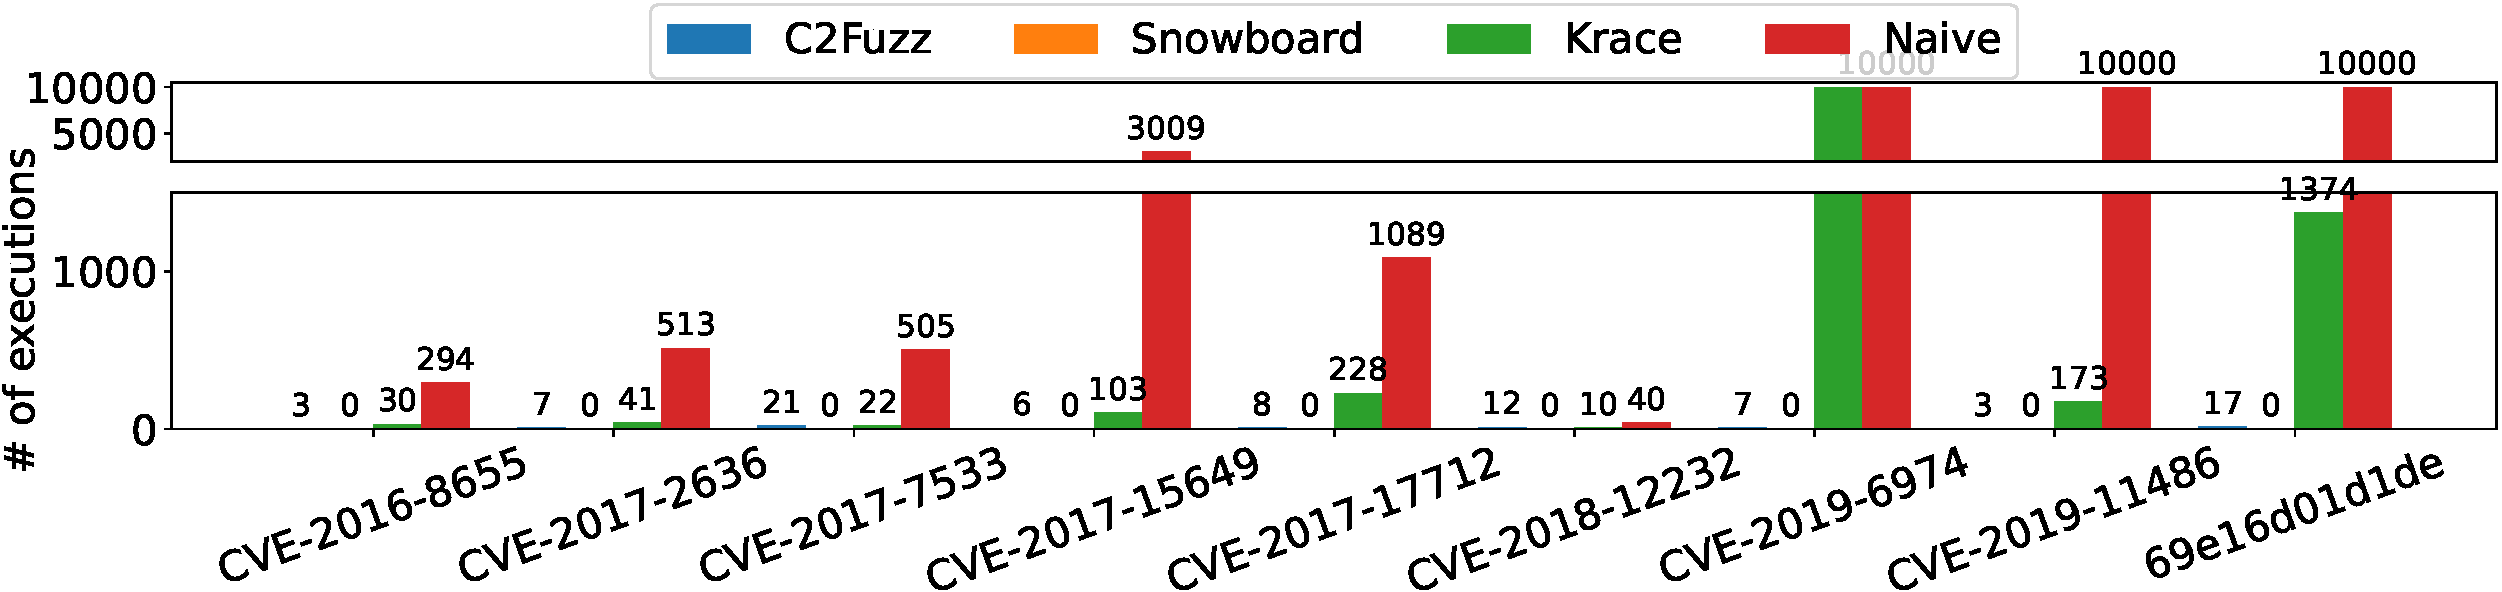
\includegraphics[width=\linewidth]{fig/comparison_graph-crop.pdf}
%   \caption{\dr{table is better?}}
%   \label{fig:eval:comparison}
% \end{figure*}
%
\begin{table*}
  \centering
  \newcommand\mc[1]{\multicolumn{1}{l}{#1}}  % shortcut macro

\resizebox{0.9\linewidth}{!}{
  \begin{tabular}{l S[table-format=7.0] l S[table-format=7.0] l S[table-format=7.0] l S[table-format=7.0] l}
    \toprule
    \multirow{2}{*}{\textbf{Bug ID}} & \multicolumn{2}{c}{\textbf{\sys}} & \multicolumn{2}{c}{\textbf{Snowboard}~\cite{snowboard}} & \multicolumn{2}{c}{\textbf{Krace}~\cite{krace}} & \multicolumn{2}{c}{\textbf{Naive}} \\
    \cmidrule(rl){2-3} \cmidrule(rl){4-5} \cmidrule(rl){6-7} \cmidrule(rl){8-9}
    & \mc{\# of exec.} & Elapsed time & \mc{\# of exec.} & Elapsed time & \mc{\# of exec.} & Elapsed time & \mc{\# of exec.} & Elapsed time \\
    \midrule
    CVE-2016-8655~\cite{cve20168655} & 6 & 2.2 & 12 & 4.0 & 96 & 44.2 & 270 & 85 \\
    % \midrule
    CVE-2017-2636~\cite{cve20172636} & 22 & 7.1 & 58 & 26.4 & 9 & 4.4 & 721 & 377.8 \\
    % \midrule
    CVE-2017-7533~\cite{cve20177533} & 30 & 16 & 191 & 58 & 53 & 24.2 & 274 & 83.3 \\
    % \midrule
    CVE-2017-17712~\cite{cve201717712} & 17 & 5.4 & 79 & 22.2 & 1296 & 359.3 & 1757 & 474.2 \\
    % \midrule
    CVE-2017-15649~\cite{cve201715649} & 38 & 13.2 & 31 & 10.0 & 342 & 100.0 & 1852 & 460.8 \\
    % \midrule
    CVE-2018-12232~\cite{cve201812232} & 12 & 3.3 & 8 & 2.4 & 14 & 4.0 & 78 & 29.1 \\
    % \midrule
    CVE-2019-6974~\cite{cve20196974} & 81 & 52.4 & 229 & 139.4 & >10000 & >5720.1 & >10000 & >5578 \\
    % \midrule
    CVE-2019-11486~\cite{cve201911486} & 3 & <1 & 37 & 16.6 & 494 & 222.6 & >10000 & >3810 \\
    % \midrule
    69e16d01d1de~\cite{snowboardbug} & 41 & 23.2 & 156 & 61.8 & >10000 & >3410.5 & >10000 & >3358 \\
    \bottomrule
  \end{tabular}
}

%%% Local Variables:
%%% mode: latex
%%% TeX-master: "../p"
%%% End:

  \caption{Result of the comparison study against various
    state-of-the-art kernel concurrency fuzzers (\ie,
    Krace~\cite{krace} and Snowboard~\cite{snowboard}). We measure the
    number of executions and the elapsed time (secs) required to
    discover each concurrency bug. The \texttt{Naive} column indicates
    the kernel's scheduler (\ie, no thread scheduling control applied).}
  \label{table:comparison-interleaving-search}
\end{table*}
%
One could argue that even if interleaving segment coverage is
informative in describing unique behaviors of offending thread
interleavings, its search space is too large to explore, and thus, it
is impractical.
%
However, it is tractable to track interleaving segment coverage with
our speculative interleaving exploration. To demonstrate this, we
compare the speculative interleaving
exploration~\autoref{ss:scheduler} against various interleaving
exploration methods proposed in prior approaches.

\PP{Comparison target}
%
We compare \sys to state-of-the-art kernel concurrency fuzzers,
Snowboard~\cite{snowboard}, and Krace~\cite{krace}.
%
Unfortunately, we cannot directly run Snowboard and Krace for the
comparison study because Krace is implemented only for file systems,
and Snowboard requires significant modifications according to our
purpose\dr{}.
%
Therefore, we implement their approaches on the multi-thread fuzzing
phase~(\autoref{sss:multithreadfuzzing}) of \sys by applying 1) the
random delay injection scheme of Krace, and 2) the
enforcing-single-interleaving-order scheme of Snowboard.
%
In addition of recent concurrency fuzzing works, we also compare with
the kernel scheduler (\ie, no thread scheduling control applied) as
the baseline.




% %
% Arguably, the most straightforward metric to compare fuzzing
% techniques is the elapsed time until concurrency bugs are discovered.
% %
% However, the elapsed time heavily depends on the randomness;
% \dr{because a fuzzer generates an input program very randomly, it is
%   possible that one fuzzer quickly generates an input program that
%   causes a concurrency bug, while another fuzzer takes very long time
%   to generate the input program}.

% In order to minimize the impact of the randomness and to concentrate
% on the performance impact of scheduling mechanisms, we predefine a
% multi-thread input as shown in \autoref{fig:multithreadinput}, and let
% a fuzzer repeatedly execute the given multi-thread input without
% generating new inputs nor mutating syscalls in the given input.

% In addition, previous fuzzing approaches

\PP{Result}
%
\autoref{table:comparison-interleaving-search} shows the comparison
result.
%
In this table, \texttt{\sys}, \texttt{Snowboard}, and \texttt{Krace}
columns display the number of executions and the elapsed time taken by
their corresponding works, and the \texttt{Naive} column corresponds
to the kernel scheduler without any thread scheduling control enabled.
%

%
Looking at the \texttt{Naive} column, we can identify the difficulty
of discovering varies from bug to bug.
%
For example, CVE-2018-12232 appears as the easiest concurrency bug to
discover since it can be discovered within 78 executions even with the
kernel scheduler.
%
On the other hand, the kernel scheduler fails to discover three
concurrency bugs, CVE-2019-6974, CVE-2019-11486, and
\texttt{69e16d01d1de} within 10K times of executions.
%
Regardless of the difficulty of discovering, \sys can discover all of
concurrency bugs very effectively.
%
\sys can discover given concurrency bugs in just 26.8 runs on average,
ranging from 3 to 81.
%
Whereas, Snowboard discovers concurrency bugs in 89 runs on average,
ragning from 8 to 229, and Krace discovers them in 329.1 runs on
average if successful, raning from 9 to 1296. Moreover, Krace even
suffers from discovering CVE-2019-6974 and \texttt{69e16d01d1de}.
%
Throughout this evaluation, we confirm that the \sys's speculative
interleaving exploration can manage the search complexity of
interleaving segment coverage, and consequently, \sys can tirgger
given concurrency bugs even much faster than previous approaches.








\subsection{Performance characteristics of \sys}
\label{ss:characteristics}

In this subsection, we analyze various performance characteristics of
\sys to comprehend how our approach affects the fuzzing process.
%
\subsubsection{All-inclusive evaluation}
\label{sss:allinclusive}

Here, we provide performance characteristics of the whole \sys.


\PP{Coverage growth.}
%
\begin{figure}[t]
  \centering
  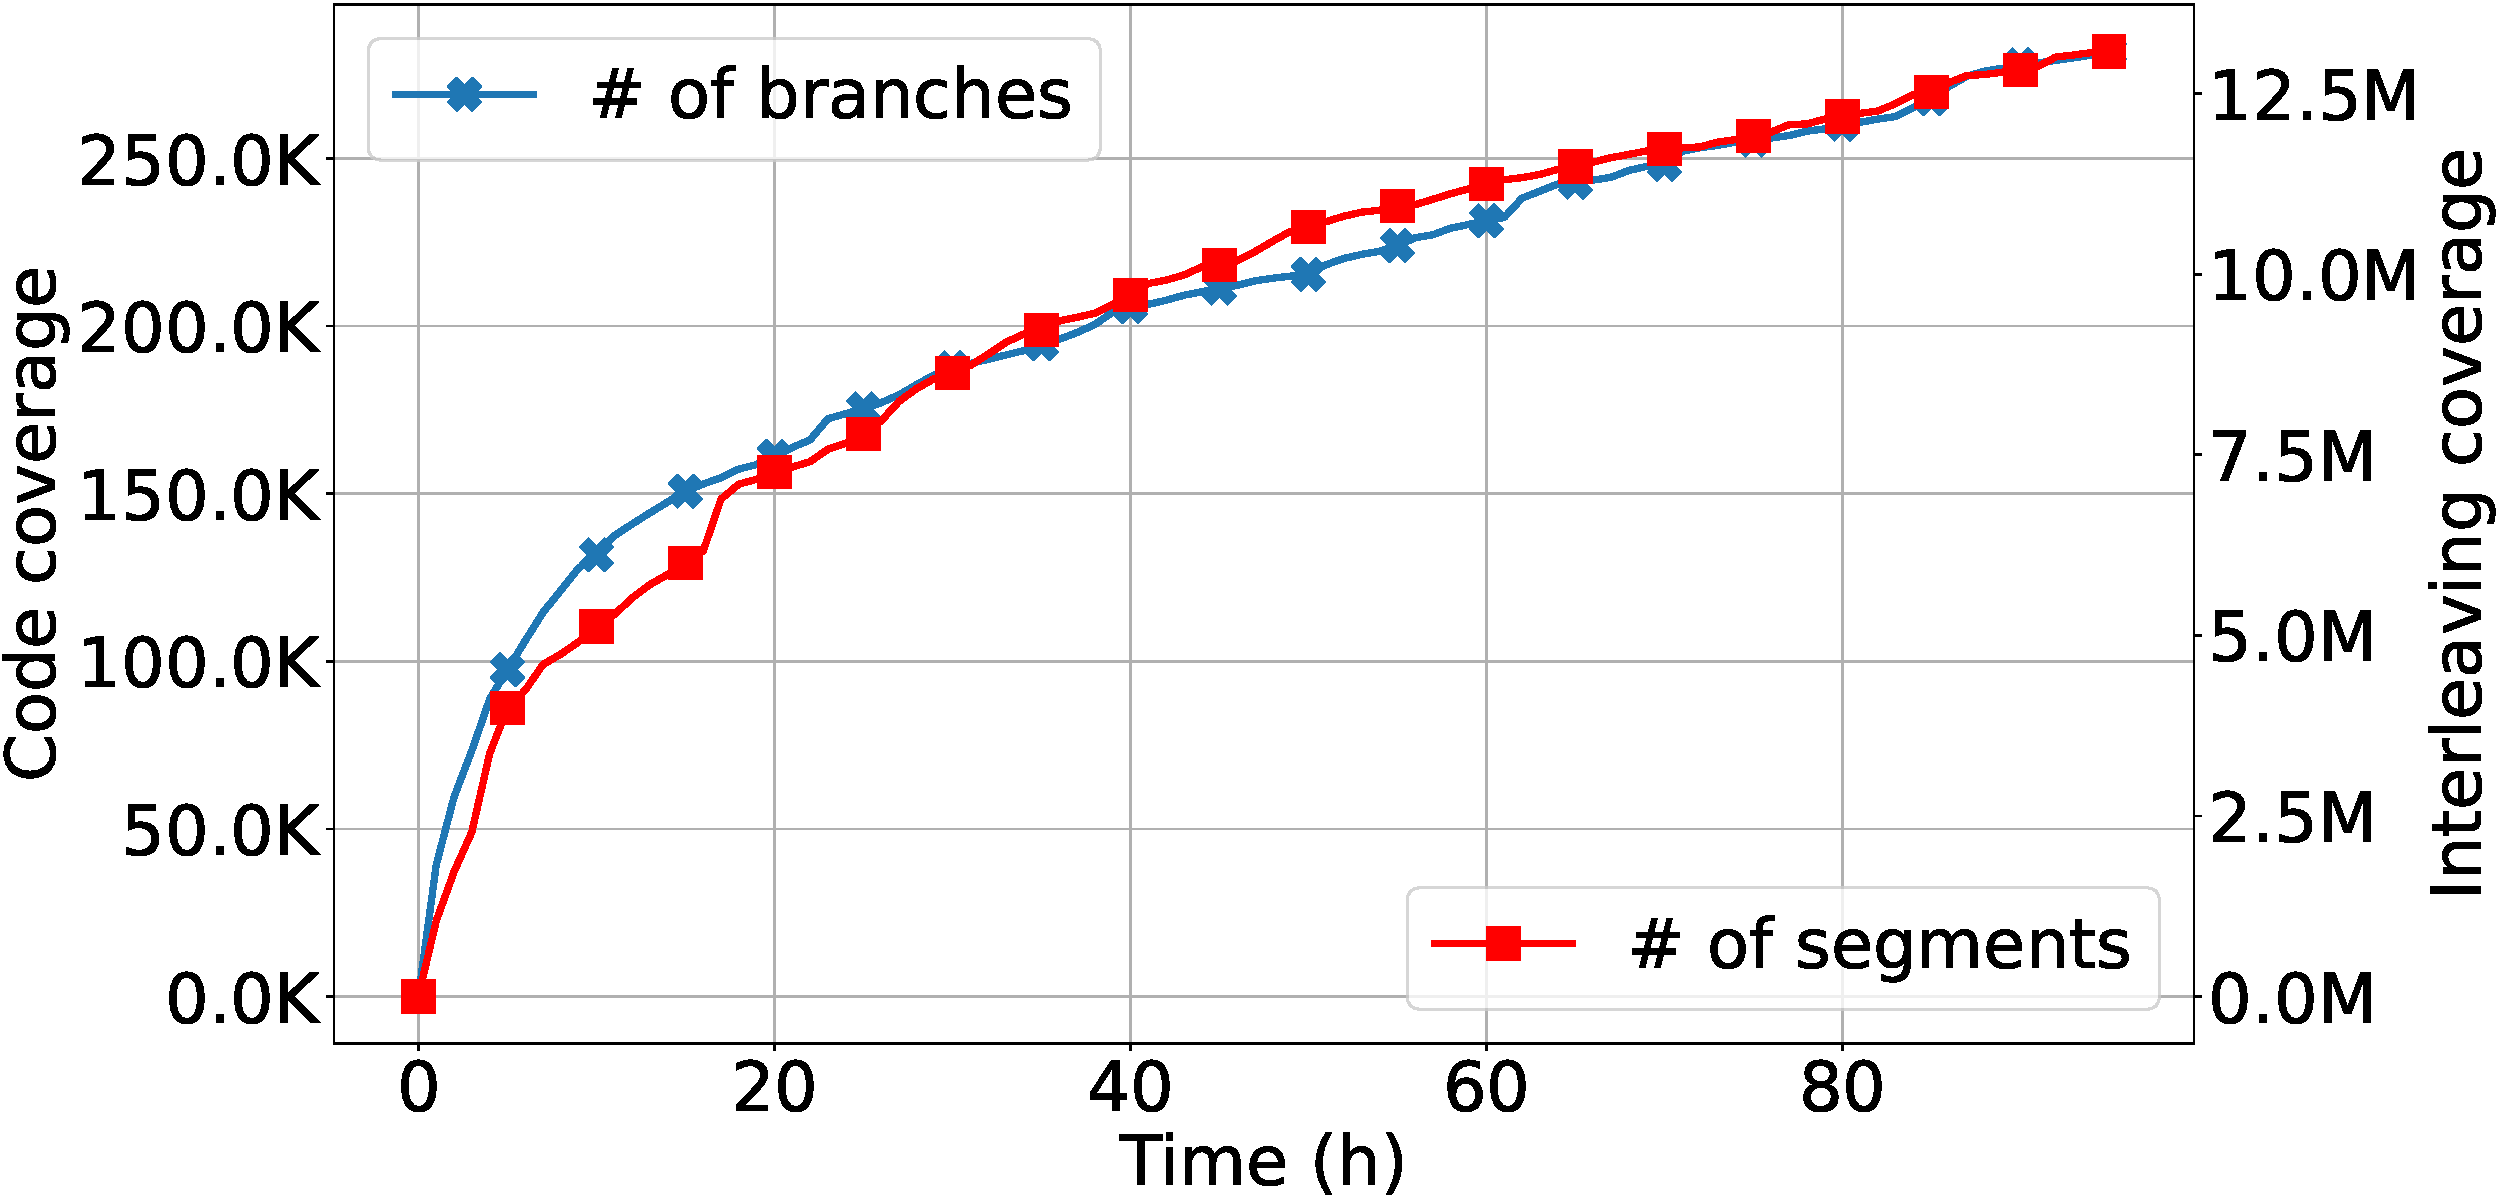
\includegraphics[width=0.9\linewidth]{fig/coverage_graph-crop.pdf}
  \caption{Coverage growth of \sys.}
  \label{fig:eval:coverage}
\end{figure}
%
Since coverage metrics are the paramount performance metric of
fuzzing, we measure the coverage growth for both code coverage (\ie,
the number of taken branches) and interelaving coverage (\ie, the
number of observed interleaving segments) during 100 hours of fuzzing.

As shown in \autoref{fig:eval:coverage}, there is a notable difference
in scale between code coverage (a line denoted by \texttt{Branch}) and
interleaving coverage (a line denoted by \texttt{Interleaving segment}).
%
While the number of taken branches just reaches to 300K, the number of
interleaving segments is over 20M. Thus, the scale of interleaving
coverage is more than 66 times of code coverage.
%
This result follows the traditional belief that the search space of
thread interleaving is very large. As a consequence, storing
interleaving segment coverage consumes more memory than storing branch
coverage.
%
In our implementation, both branch coverage and interleaving segment
coverage are represented as hash tables where each element is 8
bytes. Therefore, storing interleaving segment coverage consumes about
180\MB while storing branch coverage requires 2\MB.
%
We can consider this result as a well-known space-time
tradeoff~\cite{spacetimetradeoff}; we invest \textit{more memory} to
discover concurrency bugs \textit{faster}.
%
% In addition, considering each VM is equipped with 8\GB memory, it is
% endurable for the fuzzer to store interleaving segment coverage using
% 180\MB (or even using ten times of 180\MB).


\PP{Fuzzing throughput.}
%
\begin{table}[t]
  \small
  \centering
  \resizebox{0.65\linewidth}{!}{
\begin{tabular}{l l l}
  \toprule
  \sys & \texttt{Syzkaller} & \texttt{Syzkaller-memtrace} \\
  \midrule
  4.55 & 8.40 & 4.74 \\
  \bottomrule
\end{tabular}
}



% syzkaller: 30234
% syzkaller-memtrace: 17608
% c2fuzz: 16386


%%% Local Variables:
%%% mode: latex
%%% TeX-master: "../p"
%%% End:

  \caption{Fuzzing throughput (\# of exec/s) of \sys and
    \texttt{Syzkaller}. \texttt{Syzkaller-memtrace} indicates
    throughput of \texttt{Syzkaller} with memory access tracing
    enabled.}
  \label{table:throughput}
\end{table}
%
All \sys's mechanisms provide benefits in finding concurrency bugs
with a cost of additional overheads and throughput degradation.
%
To comprehend the trade-off, we measure the fuzzing throughput of \sys
and compare it with the \texttt{Syzkaller}'s throughput.
%
In order to experiment in the same environment, we measure throughput
with an empty set of seed. And because both \texttt{Syzkaller} and
\sys restart VMs after an hour of fuzzing, we measure throughput in an
hour of execution in order to eliminate noises caused by, for example,
VM rebooting or kernel crashes.



\autoref{table:throughput} shows the result. As expected, \sys shows
the lower throughput than \texttt{Syzkaller}. In particular, the
\sys's throughput is about 54\% of the \texttt{Syzkaller}'s
throughput.
%
To further understand why the \sys's throughput is degraded, we
additionally measure throughput of \texttt{Syzkaller} while tracing
memory accesses (through instrumentation described in
\autoref{ss:instrumentation}), but not making use of it.
%
As shown in the \texttt{Syzkaller-memtrace} column in
\autoref{table:throughput}, it shows the throughput similar to that of
\sys; the \texttt{Syzkaller-memtrace}'s throughput is just 4.1\%
higher than the throughput of \sys.


These results indicate that the throughput of \sys is mainly degraded
by the heavy instrumentation to trace memory accesses.
%
However, as Krace~\cite{krace} states, it can be understandable as the
cost for the high input quality.
%
In the fuzzer's perspective, while tracking memory accesses has
negative impacts on throughput, it provides a higher chance for a
fuzzer to execute more interesting inputs (\ie, interesting thread
interleaving) and not to waste computing resources.
%
The effectiveness of high input quality is more pronounced in
\autoref{sss:interleavingsearch}, showing \sys can discover
concurrency bugs very quickly.




\PP{Per-input overhead}
%
\begin{table}[t]
  \centering
  \resizebox{\linewidth}{!}{
  \begin{tabular}{l l l l l l }
    \toprule
    & & \multicolumn{2}{c}{Comp. overhead~(\autoref{s:design})} & \multicolumn{2}{c}{Runtime overhead~(\autoref{s:impl})} \\
    \midrule
    Total & \thead{Exec.\\syscall} & \thead{Tracking\\coverage\\(\autoref{ss:coverage})} & \thead{Interleaving\\search\\(\autoref{ss:scheduler})} & \thead{Tracing\\accsses\\(\autoref{ss:instrumentation})}  & \thead{Thread\\scheduling\\(\autoref{ss:engine})}  \\
    \midrule
    267.2 & 107.6  & 8.9 & 17.2 & 90.7 & 42.8 \\
    \bottomrule
  \end{tabular}
}

% temporary
% c2fuzz
%  execute            241116156.29326048
%  mutate             17231640.620481927
%  post               8858728.732142856
% syzkaller           107640966.51956181
% syzkaller-memtrace  198337534.77521613

%%% Local Variables:
%%% mode: latex
%%% TeX-master: "../p"
%%% End:

  \caption{
    %
    Elapsed time (ms) for executing one multi-thread input. We
    decompose the elapsed time into the system call execution
    (\texttt{Exec. syscall}), \sys's computational overheads
    (\texttt{Comp. overhead}) and runtime overhead (\texttt{Runtime
      overhead}).}
  \label{table:elapsedtime}
\end{table}
%
In \sys, there are two types of overheads for executing a single
multi-thread input, such as computational overheads, and runtime
overheads.
%
Specifically, computation overheads are caused by tracking
interleaving segment coverage after executing the
input~(\autoref{ss:coverage}), and calculating scheduling points
before executing the input~(\autoref{ss:scheduler}).
%
On the other hand, runtime overheads are caused by tracing memory
accesses~(\autoref{ss:instrumentation}) and controlling thread
scheduling~(\autoref{ss:engine}).


To closely examine these overheads, we measure the elapsed time for
executing a single multi-thread input, and break down the elapsed time
into time taken by each components (\ie, tracking interleaving segment
coverage~(\autoref{ss:coverage}), searching a thrad
interleaving~(\autoref{ss:scheduler}), tracing memory
accesses~(\autoref{ss:instrumentation}), and controlling thread
scheduling~(\autoref{ss:engine})).
%
For this measurement, we run 10 thousands times and take an average.




\autoref{table:elapsedtime} shows the result. When executing a single
input, the total elapsed time is 267.2ms.
%
During the execution, the part that took the longest time is executing
system calls; it takes 107.6ms.
%
However, overheads incurred by \sys is not negligible. Tracing memory
accesses~(\autoref{ss:instrumentation}) takes 90.7ms, and controlling
thread scheduling~(\autoref{ss:engine}) takes 42.8ms. These two
runtime overheads almost double the execution time, and are the main
cause of degrading the throughput of fuzzing as shown in the above.
%
In contrast, the total amound of time for computation is 26.1 (= 8.9 +
17.2)ms, and occupies approximately 9\% of the total elapsed time.
%
Accordingly, we can see that the computational overhead is relatively
small.



\subsubsection{Impact on coverage growth}
\label{sss:component}
%
Here, we present the impact of our design choices on both the
interleaving coverage growth and the code coverage growth.


\PP{Impact on interleaving exploration}
%
As the primiary purpose of this work is to effectively explore thread
interleavings, the \sys's approach~(\autoref{s:design}) should
contribute in effectively expanding the interleaving coverage.
%
To see how much \sys improves thread interleaving exploration, we
disable the thread scheduling control in the multi-thread fuzzing
phase of \sys, and measure the interleaving coverage.
%
The result is described in a line denoted by \texttt{Interleaivng
  segment w/o scheduling control} in \autoref{fig:eval:coverage}.
%
With the thread scheduling control disabled, \sys finds 29.1\% less
interleaving segment coverage during the same period.
%
As a consequence, we can concolude that our design choices
significantly improve in exploring thread interleavings.
%
% As a consequence, \sys can effectively discover concurrency bugs as
% shown in \autoref{ss:comparison}.



\PP{Impact on code exploration}
%
Since \sys invests the computing power to repeatedly execute a
multi-thread input (\ie, the multi-thread fuzzing phase), we expect
that \sys might explore code coverage less than the baseline
\texttt{Syzkaller}.
%
To see the difference of the code coverage exploration in \sys and
\texttt{Syzkaller}, we measure code coverage of \texttt{Syzkaller} and
illustrate it as a line denoted by \texttt{Branch (Syzkaller)} in
\autoref{fig:eval:coverage}.
%
As a result, \sys finds 3.2\% less code coverage compared to the
baseline \texttt{Syzkaller}.
%
While this is a definitely downside of \sys. However, considering the
huge benefit in exploring thread interleavings, we still believe that
this is marginal.





%%% Local Variables:
%%% mode: latex
%%% TeX-master: "p"
%%% End:
